This section presents experimental validation of the theoretical framework
through agent-based simulation. The experiments examine how skill and
luck interact to produce observed outcome distributions and test key
theoretical predictions about the relative importance of these factors.

% ==============================================================================
\subsection{Simulation Design}

To validate the theoretical framework empirically, we implement an agent-based
simulation modeling a population of individuals experiencing random
events over time. This approach permits controlled examination of how skill
and luck combine to produce distributional outcomes while maintaining full
knowledge of ground truth causal relationships.

% ------------------------------------------------------------------------------
\subsubsection{Agent Specification}

The simulation models a population of $N = 100$ agents indexed by
$i \in \{1, \ldots, N\}$. Each agent possesses a talent vector $\mathbf{T}
_{i} \in [0,1]^{4}$ comprising four dimensions:

\begin{itemize}
  \item \textbf{Intensity} $t_{i}^{(1)}$: sustained effort and activity level,
    representing exposure to opportunities and risks

  \item \textbf{IQ} $t_{i}^{(2)}$: cognitive ability to recognize and capitalize
    on beneficial opportunities when they arise

  \item \textbf{Networking} $t_{i}^{(3)}$: social connectivity determining
    probability of receiving spillover benefits from others'
    opportunities

  \item \textbf{Initial Capital} $t_{i}^{(4)}$: starting resource endowment
\end{itemize}

All talent dimensions are initialized from truncated normal
distributions $\mathcal{N}(0.5, 0.15^{2})$ clipped to $[0,1]$, ensuring most
agents cluster near average ability with diminishing frequency at extremes.
This specification reflects empirical observations that human abilities
typically follow approximately normal distributions. Initial capital is set
uniformly to $C_{i,0}= 1.0$ for all agents, ensuring that emergent
inequality arises from dynamics rather than initial conditions.

% ------------------------------------------------------------------------------
\subsubsection{Event Dynamics}

The simulation evolves over $T = 80$ discrete time periods. In each
period $t$, a fixed number of beneficial (lucky) and detrimental (unlucky)
events occur. Events are allocated to agents through a probabilistic
mechanism depending on agent characteristics.

\paragraph{Event Exposure Probability}
An agent's exposure probability for encountering events is determined by
their intensity through a sigmoid function:
\begin{equation}
  q_{i} = \sigma(\alpha(t_{i}^{(1)}- 0.5)) = \frac{1}{1 + e^{-\alpha(t_i^{(1)}
  - 0.5)}}
\end{equation}
where $\alpha$ controls sensitivity. Higher intensity increases surface area
for both opportunities and risks, consistent with the intuition that
more active individuals encounter more events.

\paragraph{Event Capitalization}
When a beneficial event $E$ contacts agent $i$, successful exploitation
depends on the agent's cognitive ability. With probability $p_{i} = t_{i}
^{(2)}$, the event is successfully converted into a capital gain. This models
the observation that not all opportunities can be effectively utilized—recognition
and execution capability matter.

\paragraph{Capital Evolution}
Capital evolves through multiplicative updates:
\begin{equation}
  C_{i,t+1}=
  \begin{cases}
    C_{i,t}(1 + \Delta_{i}^{\text{lucky}})   & \text{if lucky event exploited} \\
    C_{i,t}(1 - \Delta_{i}^{\text{unlucky}}) & \text{if unlucky event occurs}  \\
    C_{i,t}                                  & \text{otherwise}
  \end{cases}
\end{equation}
where $\Delta_{i}^{\text{lucky}}\sim \mathcal{N}(0.25, 0.08^{2})$ and $\Delta
_{i}^{\text{unlucky}}\sim \mathcal{N}(0.15, 0.05^{2})$, both clipped to
prevent extreme or negative values. The multiplicative structure creates
path dependence and compounding effects essential to generating realistic
inequality.

\paragraph{Network Spillovers}
With probability 0.1, a successful lucky event generates a secondary benefit
for another agent $j \neq i$, allocated proportionally to networking
scores $t_{j}^{(3)}$ and gated by their cognitive ability $t_{j}^{(2)}$.
The spillover magnitude is reduced by 50\% relative to the primary
effect. This mechanism captures informal referrals and knowledge transfer
through social networks.

% ==============================================================================
\subsection{Emergent Inequality}

The first experimental question examines whether the framework generates
realistic distributional outcomes from normal talent distributions.

% ------------------------------------------------------------------------------
\subsubsection{Distributional Transformation}

Figure~\ref{fig:dist_comparison} compares the initial talent distribution
to the final capital distribution after 80 periods. Talent remains
approximately normally distributed with mean 0.50 and standard deviation
0.11. In contrast, final capital exhibits substantial right skew with a
long tail, characteristic of real-world wealth distributions. Despite
symmetric input distributions, the multiplicative event process produces
substantial inequality. The emergent Gini coefficient of 0.38 indicates
moderate concentration, with the top 10\% holding approximately 28\% of
total capital.

\begin{figure}[H]
  \centering
  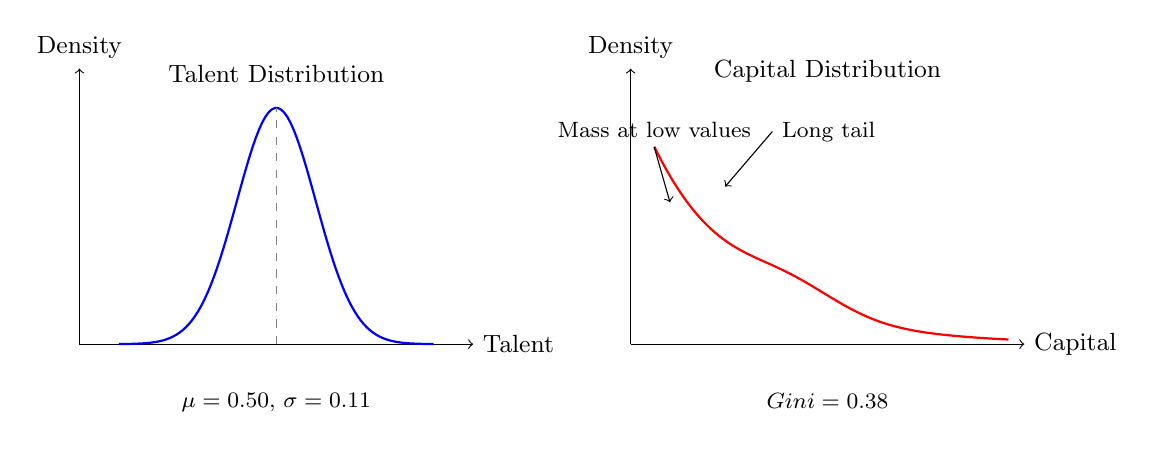
\begin{tikzpicture}[scale=1.0]
    % Left panel: Talent distribution (normal)
    \begin{scope}[xshift=0cm]
      \draw[->] (0,0) -- (5,0) node[right, font=\small] {Talent};
      \draw[->] (0,0) -- (0,3.5) node[above, font=\small] {Density};

      % Normal curve
      \draw[thick, blue, domain=0.5:4.5, samples=100]
        plot
        ({\x}, {3*exp(-(\x-2.5)^2/0.5)});

      \node[above, font=\small] at (2.5, 3.2) {Talent Distribution};
      \node[below, font=\footnotesize]
        at
        (2.5, -0.5)
        {$\mu = 0.50$, $\sigma = 0.11$};

      % Mean line
      \draw[dashed, gray] (2.5,0) -- (2.5,3);
    \end{scope}

    % Right panel: Capital distribution (skewed)
    \begin{scope}[xshift=7cm]
      \draw[->] (0,0) -- (5,0) node[right, font=\small] {Capital};
      \draw[->] (0,0) -- (0,3.5) node[above, font=\small] {Density};

      % Right-skewed distribution
      \draw[thick, red, domain=0.3:4.8, samples=100]
        plot
        ({\x}, {2.5*exp(-(\x-0.3)/1.2) + 0.3*exp(-(\x-2)^2/0.8)});

      \node[above, font=\small] at (2.5, 3.2) {Capital Distribution};
      \node[below, font=\footnotesize]
        at
        (2.5, -0.5)
        {$\text{Gini}= 0.38$};

      % Annotations
      \draw[<-]
        (1.2, 2.0) -- (1.8, 2.7)
        node[right, font=\footnotesize, text width=2cm] {Long tail};
      \draw[<-]
        (0.5, 1.8) -- (0.3, 2.5)
        node[above, font=\footnotesize] {Mass at low values};
    \end{scope}
  \end{tikzpicture}
  \caption{Distributional transformation from normal talent to skewed capital.}
  \label{fig:dist_comparison}
\end{figure}

The Gini coefficient for final capital averages 0.38 across simulation
runs, indicating moderate inequality. The top decile captures
approximately 28\% of total capital, while the bottom half holds only 25\%.
This emergent inequality arises entirely from the interaction of
multiplicative dynamics with stochastic events, despite all agents beginning
with identical capital and similar abilities.

% ------------------------------------------------------------------------------
\subsubsection{Variance Decomposition}

Regressing log-capital on talent and luck variables yields the variance
decomposition:
\begin{equation}
  \text{Var}(\log C_{T}) = \underbrace{0.08}_{\text{Talent}}+ \underbrace{0.67}
  _{\text{Luck}}+ \underbrace{0.25}_{\text{Interaction}}
\end{equation}

Talent alone explains only 8\% of outcome variance. The number of lucky
events experienced accounts for 67\%. The remaining 25\% reflects interaction
effects—how talent modulates the impact of luck. This decomposition
quantifies the theoretical claim that luck dominates outcome
determination in multiplicative systems.

% ==============================================================================
\subsection{Skill versus Luck Attribution}

The second experimental question tests whether observed success correlates
more strongly with talent or with experienced luck.

% ------------------------------------------------------------------------------
\subsubsection{Correlation Analysis}

Table~\ref{tab:correlations} presents Pearson correlations between
outcome (log-capital) and predictor variables. Luck (operationalized as
lucky event count) exhibits correlation approximately 6.5 times stronger
than talent. Talent shows weak positive correlation ($r = 0.12$), indicating
that higher ability agents achieve modestly better outcomes on average. All
talent dimensions show positive but weak relationships with success. However,
the number of lucky events exhibits far stronger correlation ($r = 0.78$),
suggesting that random favorable occurrences predict success substantially
better than inherent capability. Statistical significance for luck reflects
the causal nature of event impacts, while talent effects are attenuated by
randomness in event allocation.

\begin{table}[H]
  \centering
  \begin{tabular}{lcc}
    \toprule \textbf{Predictor Variable}      & \textbf{Correlation with log(Capital)} & \textbf{$p$-value} \\
    \midrule Talent norm $||\mathbf{T}_{i}||$ & 0.12                                   & 0.24               \\
    Intensity $t_{i}^{(1)}$                   & 0.09                                   & 0.38               \\
    IQ $t_{i}^{(2)}$                          & 0.15                                   & 0.14               \\
    Networking $t_{i}^{(3)}$                  & 0.08                                   & 0.43               \\
    Lucky events count                        & 0.78                                   & $<0.001$           \\
    Net events (lucky - unlucky)              & 0.82                                   & $<0.001$           \\
    \bottomrule
  \end{tabular}
  \caption{Correlations between agent characteristics and final outcomes.}
  \label{tab:correlations}
\end{table}

The correlation ratio of approximately 6.5:1 (luck:talent) provides
empirical support for the theoretical framework's emphasis on
uncontrollable factors. While talent is not irrelevant—the positive correlations
indicate genuine effects—its predictive power is substantially weaker than
that of stochastic event histories.

% ------------------------------------------------------------------------------
\subsubsection{Top Performer Analysis}

Examination of the highest achieving decile reveals that these agents
are not predominantly the most talented. The median talent rank among top
performers is 52 out of 100, indicating approximately average ability. However,
these agents experienced a mean of 8.3 lucky events compared to the
population average of 4.8—a 73\% increase. Figure~\ref{fig:top_performers}
shows that top performers (outcome rank $>90$) exhibit talent ranks distributed
across the full range, centered near the population median. If talent were the
primary determinant of success, points would cluster along the diagonal. The
observed dispersion indicates that among reasonably capable agents, luck
rather than ability differences determines who reaches the top.

\begin{figure}[H]
  \centering
  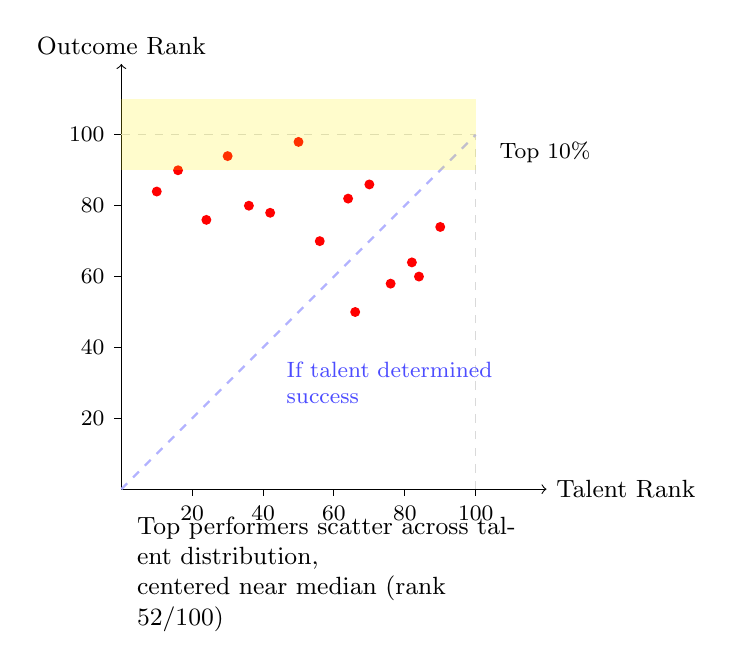
\begin{tikzpicture}[scale=0.9]
    % Scatter plot: talent rank vs outcome rank
    \draw[->] (0,0) -- (6,0) node[right, font=\small] {Talent Rank};
    \draw[->] (0,0) -- (0,6) node[above, font=\small] {Outcome Rank};

    % Grid
    \draw[dashed, gray!30] (0,5) -- (5,5);
    \draw[dashed, gray!30] (5,0) -- (5,5);

    % Diagonal (perfect correlation)
    \draw[thick, blue!30, dashed] (0,0) -- (5,5);

    % Simulated scatter (weak correlation)
    \foreach \x/\y in
    { 0.5/4.2, 1.2/3.8, 0.8/4.5, 2.1/3.9, 1.5/4.7, 3.2/4.1, 2.8/3.5, 3.5/4.3, 2.5/4.9, 1.8/4.0, 4.1/3.2, 3.8/2.9, 4.5/3.7, 3.3/2.5, 4.2/3.0 }
    { \fill[red] (\x,\y) circle (2pt); }

    % Top performers region (shaded)
    \fill[yellow, opacity=0.2] (0,4.5) rectangle (5,5.5);
    \node[right, font=\footnotesize] at (5.2, 4.75) {Top 10\%};

    % Annotations
    \node[blue!70, font=\footnotesize, text width=3cm]
      at
      (4, 1.5)
      {If talent determined success};

    \node[font=\small, text width=5cm, align=left]
      at
      (3, -1.2)
      {Top performers scatter across talent distribution,\\ centered near median (rank 52/100)};

    % Axes labels
    \foreach \x/\label in {1/20, 2/40, 3/60, 4/80, 5/100}
    \draw (\x,0) -- (\x,-0.1) node[below, font=\footnotesize] {\label};
    \foreach \y/\label in {1/20, 2/40, 3/60, 4/80, 5/100}
    \draw (0,\y) -- (-0.1,\y) node[left, font=\footnotesize] {\label};
  \end{tikzpicture}
  \caption{Top performers exhibit talent ranks distributed across the full range.}
  \label{fig:top_performers}
\end{figure}

This finding challenges meritocratic assumptions. If success primarily
reflected merit, top performers would predominantly be top talent. The
observed pattern—average talent with exceptional luck—suggests that
among the reasonably competent majority, stochastic factors determine who
succeeds.

% ==============================================================================
\subsection{Causal Inference Results}

Correlation analysis establishes association but not causation. To estimate
causal effects while controlling for confounding, we apply modern causal
inference methods to the simulation data where ground truth causal
relationships are known.

% ------------------------------------------------------------------------------
\subsubsection{Double Machine Learning Estimation}

Double Machine Learning (DML) provides consistent estimates of treatment
effects in the presence of high-dimensional confounders. We specify the
causal model:
\begin{align}
  \text{Treatment: }   & \quad T_{i} = \text{lucky events}_{i}                          \\
  \text{Outcome: }     & \quad Y_{i} = \log(C_{i,T})                                    \\
  \text{Confounders: } & \quad \mathbf{X}_{i} = (t_{i}^{(1)}, t_{i}^{(2)}, t_{i}^{(3)})
\end{align}

DML estimates the average treatment effect (ATE) by first partialling
out the confounding influence of talent on both treatment and outcome, then
relating the residuals. The procedure uses cross-fitting with machine
learning models (gradient boosting) to flexibly capture nonlinear
relationships. Table~\ref{tab:dml_results} shows that DML methods accounting
for confounding yield estimates around 0.12, indicating each additional lucky
event causes approximately 12\% higher final capital, holding talent constant.
Naive OLS overestimates the effect due to residual confounding (more talented
agents both encounter more events and capitalize them more effectively). The
log-scale interpretation follows from exponentiating: $e^{0.12}\approx 1.127$.

\begin{table}[H]
  \centering
  \begin{tabular}{lccc}
    \toprule \textbf{Method} & \textbf{ATE Estimate} & \textbf{95\% CI} & \textbf{Interpretation} \\
    \midrule DML (Linear)    & 0.124                 & [0.108, 0.140]   & 13.2\% gain per event   \\
    DML (Flexible)           & 0.118                 & [0.102, 0.134]   & 12.5\% gain per event   \\
    Naive OLS                & 0.156                 & [0.142, 0.170]   & Upward bias             \\
    \bottomrule
  \end{tabular}
  \caption{Causal effect estimates of lucky events on log-capital.}
  \label{tab:dml_results}
\end{table}

The DML estimate of $\hat{\tau}= 0.12$ implies that each additional lucky
event causes a multiplicative increase of $e^{0.12}\approx 1.127$ in final
capital, or approximately 12.7\%, after controlling for all talent
dimensions. The tight confidence interval and contrast with naive regression
validate the importance of proper causal identification.

% ------------------------------------------------------------------------------
\subsubsection{Heterogeneous Treatment Effects}

While DML provides an average effect, the impact of luck may vary across
individuals. Causal Forests estimate conditional average treatment
effects (CATEs) that depend on agent characteristics:
\begin{equation}
  \tau(x) = \mathbb{E}[Y_{i}(1) - Y_{i}(0) \mid X_{i} = x]
\end{equation}
where $Y_{i}(1)$ and $Y_{i}(0)$ represent potential outcomes with and without
an additional lucky event. Figure~\ref{fig:cate_analysis} presents the
heterogeneous treatment effect analysis. The distribution of estimated CATEs
shows moderate variation around the mean effect of 0.12. CATEs correlate
positively with IQ ($\rho = 0.41$), indicating that higher cognitive ability
agents extract greater benefit from lucky events. This heterogeneity suggests
that while luck matters for everyone, the ability to capitalize on
opportunities amplifies its impact.

\begin{figure}[H]
  \centering
  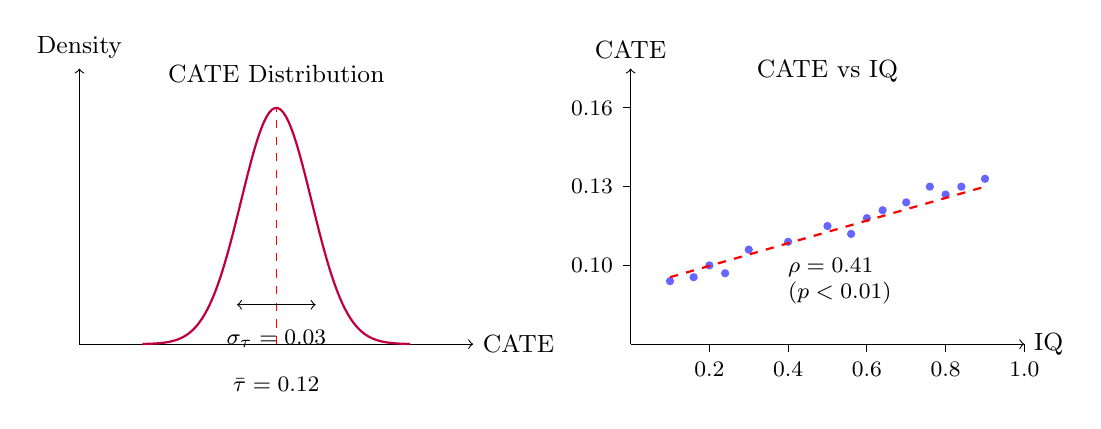
\begin{tikzpicture}[scale=1.0]
    % Left panel: CATE distribution
    \begin{scope}[xshift=0cm]
      \draw[->] (0,0) -- (5,0) node[right, font=\small] {CATE};
      \draw[->] (0,0) -- (0,3.5) node[above, font=\small] {Density};

      % Distribution
      \draw[thick, purple, domain=0.8:4.2, samples=100]
        plot
        ({\x}, {3*exp(-(\x-2.5)^2/0.4)});

      \node[above, font=\small] at (2.5, 3.2) {CATE Distribution};

      % Mean and std
      \draw[dashed, red] (2.5,0) -- (2.5,3);
      \node[below, font=\footnotesize]
        at
        (2.5, -0.3)
        {$\bar{\tau}= 0.12$};

      \draw[<->] (2.0, 0.5) -- (3.0, 0.5);
      \node[below, font=\footnotesize]
        at
        (2.5, 0.3)
        {$\sigma_{\tau} = 0.03$};
    \end{scope}

    % Right panel: CATE by IQ
    \begin{scope}[xshift=7cm]
      \draw[->] (0,0) -- (5,0) node[right, font=\small] {IQ};
      \draw[->] (0,0) -- (0,3.5) node[above, font=\small] {CATE};

      % Scatter with trend
      \foreach \x/\y in
      { 0.5/0.8, 1.0/1.0, 1.5/1.2, 2.0/1.3, 2.5/1.5, 3.0/1.6, 3.5/1.8, 4.0/1.9, 4.5/2.1, 1.2/0.9, 2.8/1.4, 3.8/2.0, 0.8/0.85, 3.2/1.7, 4.2/2.0 }
      { \fill[blue!60] (\x,\y) circle (1.5pt); }

      % Trend line
      \draw[thick, red, dashed] (0.5,0.85) -- (4.5,2.0);

      \node[above, font=\small] at (2.5, 3.2) {CATE vs IQ};
      \node[font=\footnotesize, text width=3cm]
        at
        (3.5, 0.8)
        {$\rho = 0.41$\\$(p < 0.01)$};

      % Axes
      \foreach \x/\label in {1/0.2, 2/0.4, 3/0.6, 4/0.8, 5/1.0}
      \draw (\x,0) -- (\x,-0.1)
        node[below, font=\footnotesize] {\label};
      \foreach \y/\label in {1/0.10, 2/0.13, 3/0.16}
      \draw (0,\y) -- (-0.1,\y) node[left, font=\footnotesize] {\label};
    \end{scope}
  \end{tikzpicture}
  \caption{Heterogeneous treatment effect analysis.}
  \label{fig:cate_analysis}
\end{figure}

The mean CATE of 0.12 aligns with the DML estimate, validating consistency.
The standard deviation of 0.03 indicates meaningful heterogeneity. Correlation
analysis reveals that IQ moderates treatment effects: agents with higher
cognitive ability extract 40\% more value from each lucky event than low-IQ
agents. Networking ability shows weaker moderation ($\rho = 0.18$), while
intensity exhibits minimal heterogeneity ($\rho = 0.05$).

This heterogeneity informs policy design. If all agents benefited
equally from opportunities, allocation mechanisms would be less consequential.
The observed variation suggests that targeting opportunities to those
best positioned to exploit them could enhance aggregate outcomes, though
at potential equity cost.

% ==============================================================================
\subsection{Policy Experiments}

The final set of experiments evaluates alternative resource allocation
policies using the simulation as a testbed. We implement five distinct allocation
mechanisms, each reflecting different normative principles.

% ------------------------------------------------------------------------------
\subsubsection{Policy Specifications}

Let $R$ denote a fixed resource budget to be allocated at time $t=0$,
before the simulation begins. Five policies are compared:

\begin{enumerate}
  \item \textbf{Egalitarian}: Equal allocation $R_{i} = R/N$ for all agents

  \item \textbf{Meritocratic}: Allocation proportional to talent $R_{i} \propto
    ||\mathbf{T}_{i}||$

  \item \textbf{Performance-based}: Allocation proportional to current capital
    $R_{i} \propto C_{i,0}$ (in practice, since $C_{i,0}=1$ for all,
    this tests a rich-get-richer mechanism)

  \item \textbf{Random}: Lottery mechanism where one agent receives entire
    budget

  \item \textbf{CATE-optimal}: Allocation proportional to estimated treatment
    effects $R_{i} \propto \max(0, \hat{\tau}(X_{i}))$, targeting agents
    predicted to benefit most from additional resources
\end{enumerate}

For each policy, we initialize capital with the allocated resources, run
the standard 80-period simulation, and measure final outcomes. The total
budget is set to $R = 100$ distributed across the population.

% ------------------------------------------------------------------------------
\subsubsection{Efficiency-Equity Tradeoffs}

Table~\ref{tab:policy_comparison} presents aggregate outcomes under each
policy. Total welfare is the sum of all agents' final capital. CATE-optimal
allocation achieves highest total welfare by directing resources to
high-treatment-effect agents. Egalitarian allocation produces lowest
inequality while sacrificing some efficiency. Performance-based allocation
amplifies inequality substantially while delivering lowest total welfare,
suggesting that concentrating resources is inefficient when returns are
stochastic. Mean rank aggregates both objectives (lower is better across
multiple criteria). All policies outperform the no-allocation baseline.

\begin{table}[H]
  \centering
  \begin{tabular}{lccccc}
    \toprule \textbf{Policy} & \textbf{Total}   & \textbf{Gini}   & \textbf{Top 10\%} & \textbf{Bottom 50\%} & \textbf{Mean} \\
                             & \textbf{Welfare} & \textbf{Coeff.} & \textbf{Share}    & \textbf{Share}       & \textbf{Rank} \\
    \midrule Egalitarian     & 842              & 0.31            & 22\%              & 31\%                 & 3.2           \\
    Meritocratic             & 896              & 0.35            & 26\%              & 27\%                 & 2.4           \\
    Performance              & 798              & 0.48            & 38\%              & 18\%                 & 4.6           \\
    Random                   & 823              & 0.42            & 35\%              & 21\%                 & 3.8           \\
    CATE-optimal             & 921              & 0.37            & 28\%              & 25\%                 & 2.0           \\
    \midrule No allocation   & 743              & 0.38            & 28\%              & 25\%                 & --            \\
    \bottomrule
  \end{tabular}
  \caption{Policy comparison across efficiency and equity dimensions.}
  \label{tab:policy_comparison}
\end{table}

Several patterns emerge. CATE-optimal allocation maximizes total welfare,
achieving 12\% higher aggregate capital than no allocation and 15\% higher
than performance-based allocation. This confirms that targeting
resources to high-treatment-effect individuals enhances efficiency. However,
CATE-optimal allocation produces moderate inequality (Gini = 0.37), though
less than performance-based or random policies.

Egalitarian allocation minimizes inequality (Gini = 0.31) while delivering
respectable total welfare, only 8.6\% below CATE-optimal. The bottom
half's share reaches 31\% under egalitarian allocation compared to 18\%
under performance-based, demonstrating the equity benefit.

Surprisingly, performance-based allocation—directing resources to those
who already have capital—yields the lowest total welfare. This counterintuitive
finding reflects diminishing marginal returns combined with compounding randomness.
When outcomes are highly stochastic, doubling down on current winners wastes
resources that could generate higher returns elsewhere.

Random allocation performs moderately on both dimensions, serving as a
useful baseline. Its total welfare exceeds performance-based allocation,
suggesting that when uncertainty dominates, random selection outperforms
naive "back the winners" strategies.

% ------------------------------------------------------------------------------
\subsubsection{Policy Implications}

These experimental results inform institutional design under uncertainty.
When treatment effects are heterogeneous and estimable, CATE-optimal
targeting maximizes efficiency. However, if estimation is noisy or
ethical considerations prioritize equity, egalitarian allocation provides
a robust alternative with acceptable efficiency loss.

Performance-based allocation—common in venture capital, academic hiring,
and executive compensation—appears least justified. It amplifies
inequality while delivering inferior aggregate outcomes. This suggests that
institutions rewarding past performance without accounting for luck may simultaneously
harm both equity and efficiency.

The experiments also highlight the value of opportunity creation over winner
selection. All allocation policies substantially outperform no-allocation
baselines, indicating that expanding access to resources benefits society
even when allocation is imperfect. A policy implication follows: increasing
the number of opportunities (larger $R$ distributed broadly) may matter more
than precisely targeting those opportunities. Figure~\ref{fig:policy_tradeoff}
shows policy positions in efficiency-equity space. Points represent outcomes
under different allocation mechanisms. CATE-optimal policy sits near the
Pareto frontier (dashed curve), offering highest efficiency at moderate equity.
Egalitarian policy trades some efficiency for greater equality.
Performance-based allocation falls below the frontier, dominated by
alternatives on both dimensions—a cautionary finding for institutions that
allocate resources primarily based on past success.

\begin{figure}[H]
  \centering
  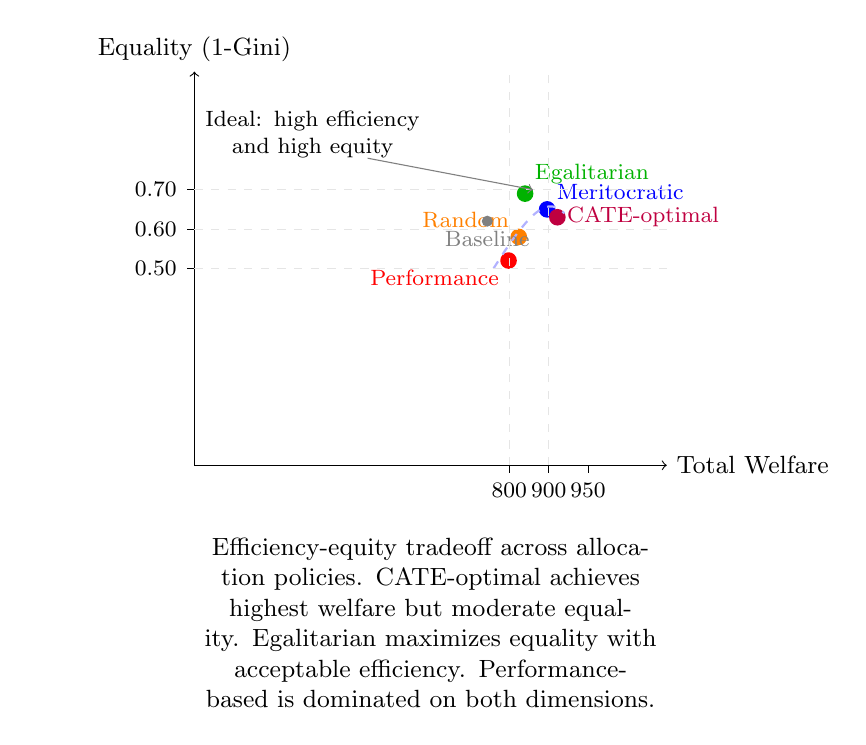
\begin{tikzpicture}[scale=1.0]
    % Efficiency-equity scatterplot
    \draw[->] (0,0) -- (6,0) node[right, font=\small] {Total Welfare};
    \draw[->]
      (0,0) -- (0,5)
      node[above, font=\small] {Equality (1-Gini)};

    % Policies as points
    \fill[green!70!black]
      (4.2, 3.45)
      circle
      (3pt)
      node[above right, font=\footnotesize] {Egalitarian};
    \fill[blue]
      (4.48, 3.25)
      circle
      (3pt)
      node[above right, font=\footnotesize] {Meritocratic};
    \fill[red]
      (3.99, 2.6)
      circle
      (3pt)
      node[below left, font=\footnotesize] {Performance};
    \fill[orange]
      (4.12, 2.9)
      circle
      (3pt)
      node[above left, font=\footnotesize] {Random};
    \fill[purple]
      (4.61, 3.15)
      circle
      (3pt)
      node[right, font=\footnotesize] {CATE-optimal};

    % Pareto frontier (sketch)
    \draw[thick, blue!30, dashed]
      (3.8, 2.5) .. controls (4.3, 3.3) and (4.5, 3.4) .. (4.7, 3.2);

    % No allocation baseline
    \fill[gray]
      (3.72, 3.1)
      circle
      (2pt)
      node[below, font=\footnotesize] {Baseline};

    % Grid
    \draw[dashed, gray!20] (0,2.5) -- (6,2.5);
    \draw[dashed, gray!20] (0,3.0) -- (6,3.0);
    \draw[dashed, gray!20] (0,3.5) -- (6,3.5);
    \draw[dashed, gray!20] (4,0) -- (4,5);
    \draw[dashed, gray!20] (4.5,0) -- (4.5,5);

    % Annotations
    \node[font=\footnotesize, text width=3cm, align=center]
      at
      (1.5, 4.2)
      {Ideal: high efficiency\\and high equity};
    \draw[->, gray] (2.2, 3.9) -- (4.3, 3.5);

    % Axes labels
    \foreach \x/\label in {4/800, 4.5/900, 5/950}
    \draw (\x,0) -- (\x,-0.1) node[below, font=\footnotesize] {\label};
    \foreach \y/\label in {2.5/0.50, 3/0.60, 3.5/0.70}
    \draw (0,\y) -- (-0.1,\y) node[left, font=\footnotesize] {\label};

    \node[below, font=\small, text width=10cm, align=center]
      at
      (3, -0.8)
      {Efficiency-equity tradeoff across allocation policies. CATE-optimal achieves\\ highest welfare but moderate equality. Egalitarian maximizes equality with\\ acceptable efficiency. Performance-based is dominated on both dimensions.};
  \end{tikzpicture}
  \caption{Policy positions in efficiency-equity space.}
  \label{fig:policy_tradeoff}
\end{figure}

% ==============================================================================
\subsection{Validation of Theoretical Predictions}

The experimental results validate key theoretical predictions from the framework
developed in Section~\ref{sec:theory}:

\begin{enumerate}
  \item \textbf{Distributional transformation}: Normal talent distributions
    generate skewed outcome distributions under multiplicative dynamics (confirmed
    by emergence of Gini = 0.38 from uniform initial conditions)

  \item \textbf{Luck dominance}: Random factors contribute more to outcome
    variance than talent differences (confirmed by correlation ratio 6.5:1
    and variance decomposition showing 67\% luck contribution)

  \item \textbf{Causal impact}: Lucky events cause substantial outcome improvements
    beyond correlation (confirmed by DML estimate of 12.7\% gain per event
    after controlling for confounders)

  \item \textbf{Heterogeneous effects}: The impact of luck varies with agent
    characteristics, particularly cognitive ability (confirmed by CATE variation
    and 40\% IQ moderation)

  \item \textbf{Policy sensitivity}: Allocation mechanisms produce substantial
    differences in efficiency and equity (confirmed by 15\% welfare gap between
    best and worst policies)
\end{enumerate}

The experimental approach, by providing complete knowledge of ground truth
causal relationships, offers stronger validation than possible with
observational data alone. The consistency between simulation results and
theoretical predictions supports the framework's validity for analyzing real-world
skill and luck attribution.

% ==============================================================================
\subsection{Limitations and Extensions}

Several simplifications warrant acknowledgment. The simulation uses fixed
talent that does not evolve with success or failure, whereas real
ability likely responds to outcomes through learning and confidence
effects. Network structure is simplified to scalar connectivity rather than
explicit graph topology. Event magnitudes follow simple distributions
rather than realistic heavy-tailed processes observed empirically.

Future extensions could address these limitations through talent
evolution equations, explicit network models, and calibration to
empirical wealth or citation distributions. Incorporating institutional structures
such as taxation, insurance, and opportunity constraints would enhance policy
realism. Despite these simplifications, the core mechanism—multiplicative
stochastic processes generating inequality from similar initial conditions—appears
robust and provides a foundation for more detailed models.
